\def\year{2020}\relax

\documentclass[letterpaper]{article} %DO NOT CHANGE THIS
\usepackage{aaai20}  %Required
\usepackage{times}  %Required
\usepackage{helvet}  %Required
\usepackage{courier}  %Required
\usepackage{url}  %Required
\usepackage{graphicx}  %Required
\usepackage{float}
\usepackage{hyperref} % For hyperlinks
\frenchspacing  %Required
\setlength{\pdfpagewidth}{8.5in}  %Required
\setlength{\pdfpageheight}{11in}  %Required
\setcounter{secnumdepth}{0}  
\usepackage{subfigure}

\begin{document}
% The file aaai.sty is the style file for AAAI Press 
% proceedings, working notes, and technical reports.
%
\title{Predicting the Results of NBA Games Using Machine Learning}
\author{Sam Macpherson, Konstantin Topaloglou-Mundy, Lazar Vukoje\\
\{skmacphe, ketopalo, lvukoje\}@uwaterloo.ca\\
University of Waterloo\\
Waterloo, ON, Canada\\}
\maketitle


%%%%%%%%%. Introduction %%%%%%%%%

\section{Introduction}
In recent years, the NBA has been extending its reach and attracting an increasingly larger and diverse audience. NBA games are viewable in many nations across the globe, and in the 2014-2015 season, the league featured 92 international players, hailing from 39 different countries \cite{jones2016predicting}. In 2019, an average of 15 million people---per finals game---watched Kawhi Leonard and the Toronto Raptors garner their first NBA championship \cite{gough_2019}. The American-based league, at the age of 74, now sits in fourth place among all sports leagues in the world by revenue \cite{amoros_2016}. People from all over the world enjoy watching and cheering on their favourite teams, and as the NBA increases its global presence, we see an equal increase in the revenue the league pulls, not just from broadcasts, but from fans purchasing jerseys and other merchandise as well. Over the last few years, we have seen a rise in a separate---though related---industry: sports betting. On May 14, 2018, the federal ban that was in place in the United States which prohibited betting on the outcomes of sporting events was lifted, leaving states free to decide to pass legislation to legalize sports betting \cite{licata_2019}. Since the ruling, 11 states have legalized sports betting---amoung them Nevada, Oregon, New York---and an additional 24 states are in the process of passing legislation \cite{licata_2019}. With the recent legalization efforts, the derivative industry has witnessed enormous support: over \$21 billion in total US handle (amount of money wagered) since 2018 \cite{legal_sports_report}. It goes without saying, then, that the ability to accurately predict sports results---especially with a mainstream league like the NBA---can be highly lucrative. This paper will describe our efforts to use existing game and player data in order to predict the result of future, arbitrary NBA games. We will focus on training a machine learning model using a season's worth of data as the input features. With high variance in team composition and individual player ability within the NBA from year to year, we believe it prudent to limit the input features to a single season, and use a model trained by such features to predict games from the playoffs for that season. We will take into account team statistics such as points per game, field goal percentage and turnovers. It is important to note that many other---sometimes abstract---outside factors can impact the result of a game, such as the ``home court advantage". To limit the scope of this project, we will limit our analysis to concrete statistics. \\

\section{Contributions}

Given the prior efforts made in predicting NBA results---in amateur, professional, and academic contexts---we are seeking to answer the broad question of can we do better? More specifically, we are interested in finding if our approach and methodology to this popular problem yields comparable or better results than the efforts of our contemporaries, and we will use their results as benchmarks throughout. On the topic of methodology, we plan on training two different machine learning models, each employing different algorithms. Before we can do so, however, the question of dataset acquisition becomes important. On this front, we will be making use of the NBA game data provided by \href{https://www.basketball-reference.com}{https://www.basketball-reference.com}, and we will do this using both an existing open source Python API, as well as a supplementary one, custom-built by us. Once we have formulated our training set according to our desired input features, we will use the TensorFlow Python library to train our models. This phase of the project introduces an interesting concept: what is the optimal model type to use for this problem, or in other words, which algorithm is best? This concept is obviously not unique to our problem, but the nature of our dataset and input features does generate a topic of discussion. On one hand, there will not be a large amount of training data, since we’ll be making models for individual basketball seasons rather than ones trained on multiple years of NBA games. On the other hand, the number of statistics that can be extracted from a basketball game is many, and the subset we choose for input features will not differ wildly from that total. As such, we will train both a decision tree and a neural network; the algorithms provided by TensorFlow will help make this possible. When our models have been trained and it comes time to test their abilitiy to label playoff games, we anticipate results that are within a reasonable delta of the models created in related works in the subject: A 60--70\% successful game prediction rate is desirable, with a greater than 70\% rate essentially answering our central question (from above) in the affirmative. It must be noted, however, that because our models will be trained on regular season data, but tested on playoff data, we face the risk of losing accuracy due to factors that cannot be explained by our regular season input data. Among these factors are the value of a head coach’s strategic adjustments in the midst of a playoff series, or matchup-specific factors that only become evident as the two teams play against one another several times in a row (which does not often happen in the regular season).

%%%%%%%%%. Related Work %%%%%%%%%

\section{Related Work}

The selection of variables that contribute to a basketball game has been a primary element of study in related work on this topic. The research conducted in ``Predicting Outcomes of NBA Basketball Games" (Jones) used over 20 different game statistics as features for their models, as well as four different approaches: 3-game moving average of team stats, 3-game moving median, 3-game moving weighted average, and seasonal averages. One technique of particular interest was that the statistics for a given team would not only include the teams statistics but also include the statistics of opposing teams when they played the team in question. Another interesting technique in this paper was the use of preprocessing on statistics; the author attempted to measure the significance of stats in training the models in order to eliminate statistics that were deemed to be unnecessary or insignificant. However, the author used data from the previous 3 seasons to predict NBA outcomes, which may be a faulty technique because of potentially significant changes to team rosters from season to season. In contrast, 
the authors \cite{predicting_maximum_entropy} of the paper ``Predicting the Outcome of NBA Playoffs Based on the Maximum Entropy Principle", restricted the data to only the current NBA season. They also used a different technique: a max entropy classifier. They argue that a max entropy classifier is appropriate for predicting NBA data for two reasons: the first is because it does not assume features are conditionally independent (which would be a mistake for NBA statistics), and second, because max entropy classifiers tend to perform well in situations with smaller number of samples (once again the case with NBA statistics). The methodology in their experiment was to use the stats of two NBA teams from the regular season of a given year  as features and then label the data with the results of the playoff matchup between those two teams for the same year. This approach seems more logical than what is was presented by Jones, because the personnel of a given team may change from season to season and so data from prior NBA seasons may not be of use for predicting an NBA playoff outcome. For example, it would not make sense to use the Golden State Warriors' dominant 2014-2018 seasons---where they maintained a win percentage of over 70\%---to predict the outcome of the 2019-2020 matches, where after sustaining multiple injuries and a change of roster, the Warriors struggled to maintain a win percentage of 23\%. In regards to the stats Chang et al. used, they decided to only use 14 rudimentary team stats (points, assists, steals, blocks, field goal percentages, etc.).
To further the discussion of relevant game statistics, a third paper, ``Identifying Basketball Performance Indicators in Regular Season and Playoff Games" \cite{IdentifyingBasketballPerformanceIndicatorsinRegularSeasonandPlayoffGames}, found that in regular season NBA games, the most important indicators of team victory was dominance in assists, defensive rebounds,  and successful 2 and 3-point field-goals. However, in the NBA playoffs, they found that the only strong indicator was defensive rebounding. The importance of defensive rebounding is corroborated by the work in ``Relative importance of performance factors in winning NBA games" \cite{RelativeImportanceofPerformanceFactorsinWinningNBAGamesinRegularSeasonversusPlayoffs}, and the authors offer an important potential explanation for this: in the playoffs, the two competing teams likely have similar shooting efficiency. This insight could be important for our work, as there will likely be matchups where a conceptual ``tiebreaker" is needed to increase the accuracy of the prediction, and this stat is evidently a candidate.

%%%%%%%%%. Methodology %%%%%%%%%

\section{Methodology}

\subsection{Evaluation Method} \label{evaluation-method}

The goal of our application is to train a model using statistics from NBA season games, and then use the model to predict the outcomes of playoff games for the same season. We will therefore need to build our training data set from the entries for the season games of each NBA team from \href{https://www.basketball-reference.com}{https://www.basketball-reference.com}, using an HTML scraper application. Thanks to the work of GitHub user jaebradley, we have just such an application, in the form of an open-source Python API: \href{https://github.com/jaebradley/basketball_reference_web_scraper}{Basketball Reference Web Scraper}. Among the functionalities of the API are the ability to pull the game schedule for a given season, the box score averages for a given team, and the box scores/outcomes of specific games. Since we would like to predict playoff outcomes, our input examples will be of the form: team 1 season averages, team 2 season averages, averages of the box scores for team 1 and 2 in the games they play during the regular season, and the label will be the winner of their matchup in the playoffs: 0 if team 1 won the series, 1 otherwise. In order to construct the training data set we require, Macpherson will write a python application which determines the winners of playoff matchups, iterates through the scheduled games in a season for the teams involved in the series, and creates a training example composed of the teams’ statistics and the series’ outcome. This way, our model will be trained using the team matchup, and the outcome of the playoff series, correlating box score averages in specific matchups to playoff outcomes. In terms of our validation set, we will use a split of 80\% training data to 20\% testing data. The API does not provide the functionality to pull data from playoff games, nor the functionality to compute average box scores of a team across a set of games, but Macpherson will write a playoff series and game matchup box score HTML scraper using the same techniques presented by the source code of GitHub user jaebradley---most notably the ``html", ``requests", and ``BeautifulSoup" Python modules. \\ \\ 
The entries in the playoff data provided by Basketball Reference are listed in an HTML table, and displayed in the form ``$<$Winning team name$>$ over $<$Losing team name$>$ (4-x)" where x is the number of games the series loser was able to win in the 7 game series. Therefore our custom HTML scraper will pull the two team names, and determine the outcome based on the ordering of the teams. Box score entries for a specific game are listed on one HTML page, in two different tables, so for each playoff series, we will scrape the box scores for all of the games the two teams played against eachother, sum them all to form an aggregate, and compute the average scores by dividing each sum by the number of these games. \\ \\
It is generally reasonable to consider the outcome of a series to be similar to performance of a team during the regular season against various teams. We will keep the scope of our model manageable by not accounting for abstract factors which contribute to the outcomes of playoff games, such as spontaneous injuries, home court advantage, and the like, because these are far too difficult to represent given NBA game data, and injuries are often impossible to predict. Writing a python application to use jaebradley’s API and the scraped HTML of playoff games and specific season matchups to build a training set is an achievable goal because the work consists of mostly list manipulation, for which Python is exceptionally powerful. Writing and debugging the application will probably take around 6 hours. We will evaluate the effectiveness of our algorithms by using prediction accuracy on the validation set. For this analysis, Macpherson will write a simple Python application which runs the validation set through our models, and compares the outputs to the actual playoff outcomes to produce the prediction accuracy. The validation application will take very little time to implement.

\subsection{Algorithms}

We are planning to test two different algorithms on our dataset and compare the relative merits of each. These two algorithms are a boosted decision tree (BDT) and an artificial neural network (NN). The BDT algorithm extends the concept of a decision tree using a technique called gradient boosting. What this algorithm does is train a series of smaller decision trees sequentially, using each subsequent tree to minimize the errors of the previous tree. The result is what is referred to as a “strong learner” which we have created from a series of “weak learners” (the individual decision trees). This method of using binary trees sequentially is known to produce an effective model on relatively little data. A NN is an algorithm that attempts to mimic the way in which a human brain learns information by using a series of neurons, which are modeled using linear classifiers then joined together in layers. By combining these linear classifiers in a network (hence the name neural network), it is possible to model very complex relationships in a dataset. Parameters of the NN like number of nodes per layer and the number of layers can be modified in order to tailor the NN to model different types of data. Both of these algorithms have been chosen because they address a specific characteristic of the data-set that we will be constructing. Decisions trees are known to be effective for training models with relatively little data. We do not expect to have an extremely large data-set to train on, as the amount of data is limited by the number of NBA match-ups that have been played in past years. Therefore, a BDT algorithm may produce favorable results given our dataset. Neural networks are known to be good for handling complex data. Our problem is feature-rich, with the number of different statistics available on individual NBA match-ups as well as aggregate statistics available on NBA teams over the course of a season, we can make the individual examples in our dataset very complex. We believe that a 
NN will be well suited to handling the complex nature of our examples, and that it may also produce favorable results on our data-set. \\ \\ 
In regards to the implementation of these algorithms, we will be using the BDT and NN algorithms provided by TensorFlow. TensorFlow is one of the leading machine learning libraries, and their implementations of both these algorithms are well written, well documented, and easy to interface with, while also providing the ability to tweak and customize the algorithms to optimize them for a given dataset. Both the BDT and NN implementations provided by TensorFlow allow users to specify general hyperparameters like learning rate, as well as algorithm specific hyperparameters like max depth for the BDT and number and size of layers for the NN. The only additional implementation that will be required of us is to read our dataset into the format specified by the TensorFlow library for training on these algorithms, as well as some experimentation to determine what values for the hyperparameters will produce good results on our dataset. \\ \\	
In regards to the timeline for completing the setup for training our models we will split the work into two parts. Topaloglou-Mundy will write the python script for training the BDT, and Vukoje will write the python script for training the NN. There will be some collaboration here as the work to read the dataset into the required format for training should be the same for both the algorithms. Here are the specific details of our timeline plan:
\subsubsection{Week of June 24th - 30th}
\begin{itemize}
\item Macpherson will do some initial experiments with the API for scraping basketball stats, including adding any additional functionality to the API. Approximate workload: 6 hours.
\item Topaloglou-Mundy and Vukoje will go over tutorials on setting up TensorFlow BDT and NN respectively, and collaborate to write a spec for the format in which Macpherson should procure the data. Approximate workload: 3 hours each
\end{itemize}
\subsubsection{Week of July 1st - 7th}
\begin{itemize}
\item Macpherson will scrape the required data and format it as specified by Topaloglou-Mundy and Vukoje. Approximate workload: 3 hours.
\item Topaloglou-Mundy and Vukoje will implement python scripts for training the BDT and NN models respectively, based on data in the format they specified. Approximate workload: 3 hours each.
\end{itemize}
\subsubsection{Week of July 8th - 14th}
\begin{itemize}
\item Topaloglou-Mundy and Vukoje will use the data provided by Macpherson to train the models using the scripts they wrote. They will record the results of the training for future use. Approximate workload: 2 hours each.
\end{itemize}
\subsubsection{Week of July 15th - 22nd}
\begin{itemize}
\item Macpherson, Topaloglou-Mundy and Vukoje will collaborate to analyze and compare the results of the two models that were trained, and write the project milestone 2 that outlines these results.
\end{itemize}

%%%%%%%%%. Results %%%%%%%%%

\section{Results}

Our final dataset consisted of 644 examples, scraped from the web pages for the 1997-98 to 2018-19 NBA seasons. There are 15 playoff series' per season, and therefore we can form 2 examples per season, by flipping the ordering of team 1 and team 2. If team 1 won the series, we order the data as described in our \nameref{evaluation-method} section and label the example ``0", we then flip the ordering of the teams, creating a new example (reordered version of the first example), and label the example as ``1". Therefore we can produce 2 examples per series, netting 30 examples per season. Some matchups proved to be too challenging to scrape from our data source: \href{https://www.basketball-reference.com}{https://www.basketball-reference.com}, because of team name changes from season to season, so in total, 8 series' were ignored across the 22 seasons, costing our dataset 16 examples. \\ \\
After writing the scripts to train our BDT and our NN, we split our 644 examples into a training set and a validation set, with ratio 0.8, and with the examples shuffled before splitting. Therefore, we trained our models on a random selection of 515 examples, and produced the following results with the remaining 129 examples.
\begin{center}
\begin{tabular}{|l|c|c|} \hline
& BDT & NN \\ \hline
Accuracy & 0.860 & 0.891 \\ \hline
Precision & 0.873 & 0.900 \\ \hline
Recall & 0.846 & 0.890 \\ \hline
AUC (Area under curve) & 0.947 & 0.964 \\ \hline
Average Loss & 0.416 & 0.413 \\ \hline
\end{tabular}
\end{center}

AUC refers to the ROC (Receiver Operator Characteristic) curve, and is a common metric to use when comparing performances between different machine learning classifiers. Here are the ROC curves we generated for our two classifiers:
\begin{figure}[H]
        \center{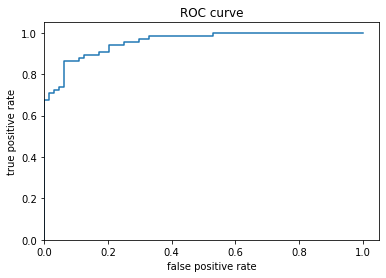
\includegraphics[width=0.4\textwidth]
        {images/BDT_ROC.png}}
        \caption{\label{fig:bdt_roc} The ROC curve for the BDT}
\end{figure}
\begin{figure}[!htb]
        \center{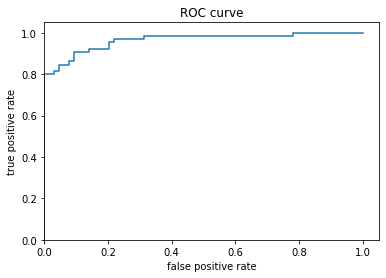
\includegraphics[width=0.4\textwidth]
        {images/NN_ROC.png}}
        \caption{\label{fig:bdt_roc} The ROC curve for the NN}
\end{figure}
Predictions produced by our models are of the form $[x,y]$, where $x$ is the probability that team 1 won the series, and $y$ is the probability that team 2 won the series. $[x,y]$ is therefore a probability distribution, which was formed by normalizing the models' ``confidence" in team 1 winning the series and team 2 winning the series. Whichever is larger of the two is the predicted winner. Therefore, another interesting metric to examine is the distribution of the probability values for $x$. Here are the corresponding plots of these probability distributions:
\begin{figure}[H]
        \center{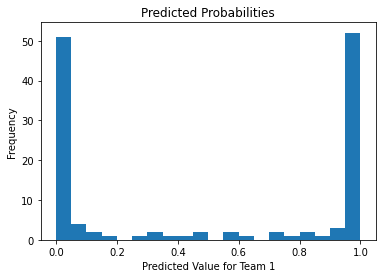
\includegraphics[width=0.35\textwidth]
        {images/BDT_prediction_probabilities.png}}
        \caption{\label{fig:bdt_prediction_distribution} The prediction probability distribution for the BDT}
\end{figure}
\begin{figure}[!htb]
        \center{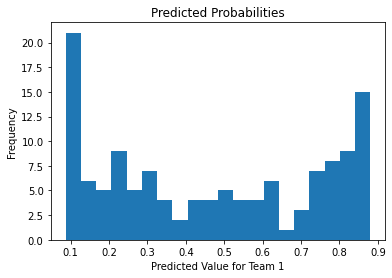
\includegraphics[width=0.35\textwidth]
        {images/NN_prediction_probabilities.png}}
        \caption{\label{fig:nn_prediction_distribution} The prediction probability distribution for the NN}
\end{figure}

Our models were trained using Google computing, with code hosted on Colab. 

%%%%%%%%%. Bibliography %%%%%%%%%
\newpage
\bibliographystyle{aaai}
\bibliography{report}

\end{document}
